\documentclass[1p]{elsarticle_modified}
%\bibliographystyle{elsarticle-num}

%\usepackage[colorlinks]{hyperref}
%\usepackage{abbrmath_seonhwa} %\Abb, \Ascr, \Acal ,\Abf, \Afrak
\usepackage{amsfonts}
\usepackage{amssymb}
\usepackage{amsmath}
\usepackage{amsthm}
\usepackage{scalefnt}
\usepackage{amsbsy}
\usepackage{kotex}
\usepackage{caption}
\usepackage{subfig}
\usepackage{color}
\usepackage{graphicx}
\usepackage{xcolor} %% white, black, red, green, blue, cyan, magenta, yellow
\usepackage{float}
\usepackage{setspace}
\usepackage{hyperref}

\usepackage{tikz}
\usetikzlibrary{arrows}

\usepackage{multirow}
\usepackage{array} % fixed length table
\usepackage{hhline}

%%%%%%%%%%%%%%%%%%%%%
\makeatletter
\renewcommand*\env@matrix[1][\arraystretch]{%
	\edef\arraystretch{#1}%
	\hskip -\arraycolsep
	\let\@ifnextchar\new@ifnextchar
	\array{*\c@MaxMatrixCols c}}
\makeatother %https://tex.stackexchange.com/questions/14071/how-can-i-increase-the-line-spacing-in-a-matrix
%%%%%%%%%%%%%%%

\usepackage[normalem]{ulem}

\newcommand{\msout}[1]{\ifmmode\text{\sout{\ensuremath{#1}}}\else\sout{#1}\fi}
%SOURCE: \msout is \stkout macro in https://tex.stackexchange.com/questions/20609/strikeout-in-math-mode

\newcommand{\cancel}[1]{
	\ifmmode
	{\color{red}\msout{#1}}
	\else
	{\color{red}\sout{#1}}
	\fi
}

\newcommand{\add}[1]{
	{\color{blue}\uwave{#1}}
}

\newcommand{\replace}[2]{
	\ifmmode
	{\color{red}\msout{#1}}{\color{blue}\uwave{#2}}
	\else
	{\color{red}\sout{#1}}{\color{blue}\uwave{#2}}
	\fi
}

\newcommand{\Sol}{\mathcal{S}} %segment
\newcommand{\D}{D} %diagram
\newcommand{\A}{\mathcal{A}} %arc


%%%%%%%%%%%%%%%%%%%%%%%%%%%%%5 test

\def\sl{\operatorname{\textup{SL}}(2,\Cbb)}
\def\psl{\operatorname{\textup{PSL}}(2,\Cbb)}
\def\quan{\mkern 1mu \triangleright \mkern 1mu}

\theoremstyle{definition}
\newtheorem{thm}{Theorem}[section]
\newtheorem{prop}[thm]{Proposition}
\newtheorem{lem}[thm]{Lemma}
\newtheorem{ques}[thm]{Question}
\newtheorem{cor}[thm]{Corollary}
\newtheorem{defn}[thm]{Definition}
\newtheorem{exam}[thm]{Example}
\newtheorem{rmk}[thm]{Remark}
\newtheorem{alg}[thm]{Algorithm}

\newcommand{\I}{\sqrt{-1}}
\begin{document}

%\begin{frontmatter}
%
%\title{Boundary parabolic representations of knots up to 8 crossings}
%
%%% Group authors per affiliation:
%\author{Yunhi Cho} 
%\address{Department of Mathematics, University of Seoul, Seoul, Korea}
%\ead{yhcho@uos.ac.kr}
%
%
%\author{Seonhwa Kim} %\fnref{s_kim}}
%\address{Center for Geometry and Physics, Institute for Basic Science, Pohang, 37673, Korea}
%\ead{ryeona17@ibs.re.kr}
%
%\author{Hyuk Kim}
%\address{Department of Mathematical Sciences, Seoul National University, Seoul 08826, Korea}
%\ead{hyukkim@snu.ac.kr}
%
%\author{Seokbeom Yoon}
%\address{Department of Mathematical Sciences, Seoul National University, Seoul, 08826,  Korea}
%\ead{sbyoon15@snu.ac.kr}
%
%\begin{abstract}
%We find all boundary parabolic representation of knots up to 8 crossings.
%
%\end{abstract}
%\begin{keyword}
%    \MSC[2010] 57M25 
%\end{keyword}
%
%\end{frontmatter}

%\linenumbers
%\tableofcontents
%
\newcommand\colored[1]{\textcolor{white}{\rule[-0.35ex]{0.8em}{1.4ex}}\kern-0.8em\color{red} #1}%
%\newcommand\colored[1]{\textcolor{white}{ #1}\kern-2.17ex	\textcolor{white}{ #1}\kern-1.81ex	\textcolor{white}{ #1}\kern-2.15ex\color{red}#1	}

{\Large $\underline{12a_{0039}~(K12a_{0039})}$}

\setlength{\tabcolsep}{10pt}
\renewcommand{\arraystretch}{1.6}
\vspace{1cm}\begin{tabular}{m{100pt}>{\centering\arraybackslash}m{274pt}}
\multirow{5}{120pt}{
	\centering
	\includegraphics[width=112pt]{../../../GIT/diagram.site/Diagrams/png/840_12a_0039.png}\\
\ \ \ A knot diagram\footnotemark}&
\allowdisplaybreaks
\textbf{Linearized knot diagam} \\
\cline{2-2}
 &
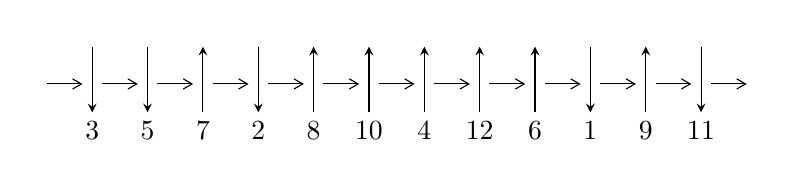
\begin{tikzpicture}[x=20pt, y=17pt]
	% nodes
	\node (C0) at (0, 0) {};
	\node (C1) at (1, 0) {};
	\node (C1U) at (1, +1) {};
	\node (C1D) at (1, -1) {3};

	\node (C2) at (2, 0) {};
	\node (C2U) at (2, +1) {};
	\node (C2D) at (2, -1) {5};

	\node (C3) at (3, 0) {};
	\node (C3U) at (3, +1) {};
	\node (C3D) at (3, -1) {7};

	\node (C4) at (4, 0) {};
	\node (C4U) at (4, +1) {};
	\node (C4D) at (4, -1) {2};

	\node (C5) at (5, 0) {};
	\node (C5U) at (5, +1) {};
	\node (C5D) at (5, -1) {8};

	\node (C6) at (6, 0) {};
	\node (C6U) at (6, +1) {};
	\node (C6D) at (6, -1) {10};

	\node (C7) at (7, 0) {};
	\node (C7U) at (7, +1) {};
	\node (C7D) at (7, -1) {4};

	\node (C8) at (8, 0) {};
	\node (C8U) at (8, +1) {};
	\node (C8D) at (8, -1) {12};

	\node (C9) at (9, 0) {};
	\node (C9U) at (9, +1) {};
	\node (C9D) at (9, -1) {6};

	\node (C10) at (10, 0) {};
	\node (C10U) at (10, +1) {};
	\node (C10D) at (10, -1) {1};

	\node (C11) at (11, 0) {};
	\node (C11U) at (11, +1) {};
	\node (C11D) at (11, -1) {9};

	\node (C12) at (12, 0) {};
	\node (C12U) at (12, +1) {};
	\node (C12D) at (12, -1) {11};
	\node (C13) at (13, 0) {};

	% arrows
	\draw[->,>={angle 60}]
	(C0) edge (C1) (C1) edge (C2) (C2) edge (C3) (C3) edge (C4) (C4) edge (C5) (C5) edge (C6) (C6) edge (C7) (C7) edge (C8) (C8) edge (C9) (C9) edge (C10) (C10) edge (C11) (C11) edge (C12) (C12) edge (C13) ;	\draw[->,>=stealth]
	(C1U) edge (C1D) (C2U) edge (C2D) (C3D) edge (C3U) (C4U) edge (C4D) (C5D) edge (C5U) (C6D) edge (C6U) (C7D) edge (C7U) (C8D) edge (C8U) (C9D) edge (C9U) (C10U) edge (C10D) (C11D) edge (C11U) (C12U) edge (C12D) ;
	\end{tikzpicture} \\
\hhline{~~} \\& 
\textbf{Solving Sequence} \\ \cline{2-2} 
 &
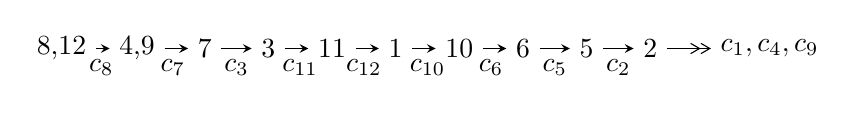
\begin{tikzpicture}[x=23pt, y=7pt]
	% node
	\node (A0) at (-1/8, 0) {8,12};
	\node (A1) at (17/16, 0) {4,9};
	\node (A2) at (17/8, 0) {7};
	\node (A3) at (25/8, 0) {3};
	\node (A4) at (33/8, 0) {11};
	\node (A5) at (41/8, 0) {1};
	\node (A6) at (49/8, 0) {10};
	\node (A7) at (57/8, 0) {6};
	\node (A8) at (65/8, 0) {5};
	\node (A9) at (73/8, 0) {2};
	\node (C1) at (1/2, -1) {$c_{8}$};
	\node (C2) at (13/8, -1) {$c_{7}$};
	\node (C3) at (21/8, -1) {$c_{3}$};
	\node (C4) at (29/8, -1) {$c_{11}$};
	\node (C5) at (37/8, -1) {$c_{12}$};
	\node (C6) at (45/8, -1) {$c_{10}$};
	\node (C7) at (53/8, -1) {$c_{6}$};
	\node (C8) at (61/8, -1) {$c_{5}$};
	\node (C9) at (69/8, -1) {$c_{2}$};
	\node (A10) at (11, 0) {$c_{1},c_{4},c_{9}$};

	% edge
	\draw[->,>=stealth]	
	(A0) edge (A1) (A1) edge (A2) (A2) edge (A3) (A3) edge (A4) (A4) edge (A5) (A5) edge (A6) (A6) edge (A7) (A7) edge (A8) (A8) edge (A9) ;
	\draw[->>,>={angle 60}]	
	(A9) edge (A10);
\end{tikzpicture} \\ 

\end{tabular} \\

\footnotetext{
The image of knot diagram is generated by the software ``\textbf{Draw programme}" developed by Andrew Bartholomew(\url{http://www.layer8.co.uk/maths/draw/index.htm\#Running-draw}), where we modified some parts for our purpose(\url{https://github.com/CATsTAILs/LinksPainter}).
}\phantom \\ \newline 
\centering \textbf{Ideals for irreducible components\footnotemark of $X_{\text{par}}$} 
 
\begin{align*}
I^u_{1}&=\langle 
-8.97511\times10^{37} u^{113}+7.35370\times10^{38} u^{112}+\cdots+2.85889\times10^{36} b+1.14745\times10^{38},\\
\phantom{I^u_{1}}&\phantom{= \langle  }-5.68472\times10^{37} u^{113}+5.72364\times10^{38} u^{112}+\cdots+2.85889\times10^{36} a+1.75186\times10^{38},\\
\phantom{I^u_{1}}&\phantom{= \langle  }u^{114}-8 u^{113}+\cdots-10 u+1\rangle \\
I^u_{2}&=\langle 
3 a^5 u+12 a^5-19 a^4 u-11 a^4-32 a^3 u+15 a^3-27 a^2 u-43 a^2-64 a u+13 b-35 a-15 u-8,\\
\phantom{I^u_{2}}&\phantom{= \langle  }a^6- a^5 u- a^5-4 a^4 u+a^4- a^3 u-2 a^3-7 a^2 u-4 a^2-3 a u- a- u,\;u^2+u+1\rangle \\
I^u_{3}&=\langle 
b,\;- u^4+u^3- u^2+a-1,\;u^9- u^8+2 u^7- u^6+3 u^5- u^4+2 u^3+u+1\rangle \\
\\
\end{align*}
\raggedright * 3 irreducible components of $\dim_{\mathbb{C}}=0$, with total 135 representations.\\
\footnotetext{All coefficients of polynomials are rational numbers. But the coefficients are sometimes approximated in decimal forms when there is not enough margin.}
\newpage
\renewcommand{\arraystretch}{1}
\centering \section*{I. $I^u_{1}= \langle -8.98\times10^{37} u^{113}+7.35\times10^{38} u^{112}+\cdots+2.86\times10^{36} b+1.15\times10^{38},\;-5.68\times10^{37} u^{113}+5.72\times10^{38} u^{112}+\cdots+2.86\times10^{36} a+1.75\times10^{38},\;u^{114}-8 u^{113}+\cdots-10 u+1 \rangle$}
\flushleft \textbf{(i) Arc colorings}\\
\begin{tabular}{m{7pt} m{180pt} m{7pt} m{180pt} }
\flushright $a_{8}=$&$\begin{pmatrix}1\\0\end{pmatrix}$ \\
\flushright $a_{12}=$&$\begin{pmatrix}0\\u\end{pmatrix}$ \\
\flushright $a_{4}=$&$\begin{pmatrix}19.8844 u^{113}-200.205 u^{112}+\cdots+518.572 u-61.2777\\31.3937 u^{113}-257.222 u^{112}+\cdots+385.856 u-40.1363\end{pmatrix}$ \\
\flushright $a_{9}=$&$\begin{pmatrix}1\\- u^2\end{pmatrix}$ \\
\flushright $a_{7}=$&$\begin{pmatrix}-51.3794 u^{113}+326.932 u^{112}+\cdots+7.96086 u-6.96895\\69.5096 u^{113}-585.675 u^{112}+\cdots+960.466 u-102.166\end{pmatrix}$ \\
\flushright $a_{3}=$&$\begin{pmatrix}64.4029 u^{113}-512.039 u^{112}+\cdots+716.519 u-81.1594\\-8.85702 u^{113}+89.4939 u^{112}+\cdots-201.213 u+22.9378\end{pmatrix}$ \\
\flushright $a_{11}=$&$\begin{pmatrix}- u\\u^3+u\end{pmatrix}$ \\
\flushright $a_{1}=$&$\begin{pmatrix}- u^3\\u^5+u^3+u\end{pmatrix}$ \\
\flushright $a_{10}=$&$\begin{pmatrix}- u^5- u\\u^7+u^5+2 u^3+u\end{pmatrix}$ \\
\flushright $a_{6}=$&$\begin{pmatrix}-22.3300 u^{113}+29.1895 u^{112}+\cdots+766.379 u-89.5923\\90.2870 u^{113}-772.336 u^{112}+\cdots+1308.83 u-139.642\end{pmatrix}$ \\
\flushright $a_{5}=$&$\begin{pmatrix}-112.617 u^{113}+801.526 u^{112}+\cdots-542.454 u+50.0496\\90.2870 u^{113}-772.336 u^{112}+\cdots+1308.83 u-139.642\end{pmatrix}$ \\
\flushright $a_{2}=$&$\begin{pmatrix}-24.7381 u^{113}+116.628 u^{112}+\cdots+306.583 u-42.8522\\64.8502 u^{113}-546.552 u^{112}+\cdots+891.089 u-94.0285\end{pmatrix}$\\&\end{tabular}
\flushleft \textbf{(ii) Obstruction class $= -1$}\\~\\
\flushleft \textbf{(iii) Cusp Shapes $= -15.7662 u^{113}+115.090 u^{112}+\cdots-86.6471 u+5.47371$}\\~\\
\newpage\renewcommand{\arraystretch}{1}
\flushleft \textbf{(iv) u-Polynomials at the component}\newline \\
\begin{tabular}{m{50pt}|m{274pt}}
Crossings & \hspace{64pt}u-Polynomials at each crossing \\
\hline $$\begin{aligned}c_{1}\end{aligned}$$&$\begin{aligned}
&u^{114}+52 u^{113}+\cdots+62 u+1
\end{aligned}$\\
\hline $$\begin{aligned}c_{2},c_{4}\end{aligned}$$&$\begin{aligned}
&u^{114}-12 u^{113}+\cdots+22 u-1
\end{aligned}$\\
\hline $$\begin{aligned}c_{3},c_{7}\end{aligned}$$&$\begin{aligned}
&u^{114}-3 u^{113}+\cdots-3072 u+512
\end{aligned}$\\
\hline $$\begin{aligned}c_{5}\end{aligned}$$&$\begin{aligned}
&u^{114}+4 u^{113}+\cdots+1228166 u-118529
\end{aligned}$\\
\hline $$\begin{aligned}c_{6},c_{9}\end{aligned}$$&$\begin{aligned}
&u^{114}-2 u^{113}+\cdots+16384 u-4096
\end{aligned}$\\
\hline $$\begin{aligned}c_{8},c_{11}\end{aligned}$$&$\begin{aligned}
&u^{114}+8 u^{113}+\cdots+10 u+1
\end{aligned}$\\
\hline $$\begin{aligned}c_{10},c_{12}\end{aligned}$$&$\begin{aligned}
&u^{114}+36 u^{113}+\cdots+10 u+1
\end{aligned}$\\
\hline
\end{tabular}\\~\\
\newpage\renewcommand{\arraystretch}{1}
\flushleft \textbf{(v) Riley Polynomials at the component}\newline \\
\begin{tabular}{m{50pt}|m{274pt}}
Crossings & \hspace{64pt}Riley Polynomials at each crossing \\
\hline $$\begin{aligned}c_{1}\end{aligned}$$&$\begin{aligned}
&y^{114}+32 y^{113}+\cdots+6582 y+1
\end{aligned}$\\
\hline $$\begin{aligned}c_{2},c_{4}\end{aligned}$$&$\begin{aligned}
&y^{114}-52 y^{113}+\cdots-62 y+1
\end{aligned}$\\
\hline $$\begin{aligned}c_{3},c_{7}\end{aligned}$$&$\begin{aligned}
&y^{114}-63 y^{113}+\cdots-9437184 y+262144
\end{aligned}$\\
\hline $$\begin{aligned}c_{5}\end{aligned}$$&$\begin{aligned}
&y^{114}-60 y^{113}+\cdots-2033070061434 y+14049123841
\end{aligned}$\\
\hline $$\begin{aligned}c_{6},c_{9}\end{aligned}$$&$\begin{aligned}
&y^{114}-70 y^{113}+\cdots-251658240 y+16777216
\end{aligned}$\\
\hline $$\begin{aligned}c_{8},c_{11}\end{aligned}$$&$\begin{aligned}
&y^{114}+36 y^{113}+\cdots+10 y+1
\end{aligned}$\\
\hline $$\begin{aligned}c_{10},c_{12}\end{aligned}$$&$\begin{aligned}
&y^{114}+92 y^{113}+\cdots+4042 y+1
\end{aligned}$\\
\hline
\end{tabular}\\~\\
\newpage\flushleft \textbf{(vi) Complex Volumes and Cusp Shapes}
$$\begin{array}{c|c|c}  
\text{Solutions to }I^u_{1}& \I (\text{vol} + \sqrt{-1}CS) & \text{Cusp shape}\\
 \hline 
\begin{aligned}
u &= \phantom{-}0.000620 + 0.995927 I \\
a &= \phantom{-}1.299800 - 0.241663 I \\
b &= \phantom{-}0.909069 - 0.395900 I\end{aligned}
 & -3.21254 - 4.24812 I & \phantom{-0.000000 } 0 \\ \hline\begin{aligned}
u &= \phantom{-}0.000620 - 0.995927 I \\
a &= \phantom{-}1.299800 + 0.241663 I \\
b &= \phantom{-}0.909069 + 0.395900 I\end{aligned}
 & -3.21254 + 4.24812 I & \phantom{-0.000000 } 0 \\ \hline\begin{aligned}
u &= -0.588448 + 0.865197 I \\
a &= -0.781789 - 0.376818 I \\
b &= \phantom{-}0.336616 - 0.121889 I\end{aligned}
 & \phantom{-}0.46811 - 2.32542 I & \phantom{-0.000000 } 0 \\ \hline\begin{aligned}
u &= -0.588448 - 0.865197 I \\
a &= -0.781789 + 0.376818 I \\
b &= \phantom{-}0.336616 + 0.121889 I\end{aligned}
 & \phantom{-}0.46811 + 2.32542 I & \phantom{-0.000000 } 0 \\ \hline\begin{aligned}
u &= \phantom{-}0.778086 + 0.701982 I \\
a &= \phantom{-}0.231260 - 0.133436 I \\
b &= -0.668937 - 0.129520 I\end{aligned}
 & \phantom{-}3.31863 - 0.81707 I & \phantom{-0.000000 } 0 \\ \hline\begin{aligned}
u &= \phantom{-}0.778086 - 0.701982 I \\
a &= \phantom{-}0.231260 + 0.133436 I \\
b &= -0.668937 + 0.129520 I\end{aligned}
 & \phantom{-}3.31863 + 0.81707 I & \phantom{-0.000000 } 0 \\ \hline\begin{aligned}
u &= -0.505823 + 0.918744 I \\
a &= \phantom{-}0.73874 - 2.25181 I \\
b &= -0.312072 - 0.402365 I\end{aligned}
 & -1.78702 - 2.46027 I & \phantom{-0.000000 } 0 \\ \hline\begin{aligned}
u &= -0.505823 - 0.918744 I \\
a &= \phantom{-}0.73874 + 2.25181 I \\
b &= -0.312072 + 0.402365 I\end{aligned}
 & -1.78702 + 2.46027 I & \phantom{-0.000000 } 0 \\ \hline\begin{aligned}
u &= \phantom{-}0.678178 + 0.804338 I \\
a &= \phantom{-}0.138606 + 0.188536 I \\
b &= \phantom{-}0.969106 - 0.620652 I\end{aligned}
 & \phantom{-}1.08443 - 3.92816 I & \phantom{-0.000000 } 0 \\ \hline\begin{aligned}
u &= \phantom{-}0.678178 - 0.804338 I \\
a &= \phantom{-}0.138606 - 0.188536 I \\
b &= \phantom{-}0.969106 + 0.620652 I\end{aligned}
 & \phantom{-}1.08443 + 3.92816 I & \phantom{-0.000000 } 0\\
 \hline 
 \end{array}$$\newpage$$\begin{array}{c|c|c}  
\text{Solutions to }I^u_{1}& \I (\text{vol} + \sqrt{-1}CS) & \text{Cusp shape}\\
 \hline 
\begin{aligned}
u &= -0.096539 + 1.054780 I \\
a &= -1.077720 - 0.337003 I \\
b &= -0.832093 - 0.241574 I\end{aligned}
 & -2.66766 - 0.82890 I & \phantom{-0.000000 } 0 \\ \hline\begin{aligned}
u &= -0.096539 - 1.054780 I \\
a &= -1.077720 + 0.337003 I \\
b &= -0.832093 + 0.241574 I\end{aligned}
 & -2.66766 + 0.82890 I & \phantom{-0.000000 } 0 \\ \hline\begin{aligned}
u &= -0.243867 + 1.045790 I \\
a &= \phantom{-}1.14280 + 1.22814 I \\
b &= -0.831060 + 0.215460 I\end{aligned}
 & -2.72201 - 3.15265 I & \phantom{-0.000000 } 0 \\ \hline\begin{aligned}
u &= -0.243867 - 1.045790 I \\
a &= \phantom{-}1.14280 - 1.22814 I \\
b &= -0.831060 - 0.215460 I\end{aligned}
 & -2.72201 + 3.15265 I & \phantom{-0.000000 } 0 \\ \hline\begin{aligned}
u &= -0.332538 + 1.023910 I \\
a &= \phantom{-}0.50463 + 1.46650 I \\
b &= -0.137018 + 0.888476 I\end{aligned}
 & -1.00115 - 1.37350 I & \phantom{-0.000000 } 0 \\ \hline\begin{aligned}
u &= -0.332538 - 1.023910 I \\
a &= \phantom{-}0.50463 - 1.46650 I \\
b &= -0.137018 - 0.888476 I\end{aligned}
 & -1.00115 + 1.37350 I & \phantom{-0.000000 } 0 \\ \hline\begin{aligned}
u &= -0.689886 + 0.597095 I \\
a &= -0.976474 + 0.359837 I \\
b &= \phantom{-}1.057270 - 0.233439 I\end{aligned}
 & \phantom{-}1.74936 - 3.74948 I & \phantom{-0.000000 } 0 \\ \hline\begin{aligned}
u &= -0.689886 - 0.597095 I \\
a &= -0.976474 - 0.359837 I \\
b &= \phantom{-}1.057270 + 0.233439 I\end{aligned}
 & \phantom{-}1.74936 + 3.74948 I & \phantom{-0.000000 } 0 \\ \hline\begin{aligned}
u &= -0.241829 + 1.089860 I \\
a &= -0.85277 - 1.16507 I \\
b &= -0.348992 - 1.012170 I\end{aligned}
 & -1.63970 - 5.47705 I & \phantom{-0.000000 } 0 \\ \hline\begin{aligned}
u &= -0.241829 - 1.089860 I \\
a &= -0.85277 + 1.16507 I \\
b &= -0.348992 + 1.012170 I\end{aligned}
 & -1.63970 + 5.47705 I & \phantom{-0.000000 } 0\\
 \hline 
 \end{array}$$\newpage$$\begin{array}{c|c|c}  
\text{Solutions to }I^u_{1}& \I (\text{vol} + \sqrt{-1}CS) & \text{Cusp shape}\\
 \hline 
\begin{aligned}
u &= \phantom{-}0.750758 + 0.827314 I \\
a &= \phantom{-}0.129507 - 0.152369 I \\
b &= -0.742772 + 0.683809 I\end{aligned}
 & \phantom{-}3.89107 + 0.23526 I & \phantom{-0.000000 } 0 \\ \hline\begin{aligned}
u &= \phantom{-}0.750758 - 0.827314 I \\
a &= \phantom{-}0.129507 + 0.152369 I \\
b &= -0.742772 - 0.683809 I\end{aligned}
 & \phantom{-}3.89107 - 0.23526 I & \phantom{-0.000000 } 0 \\ \hline\begin{aligned}
u &= -0.406450 + 0.778487 I \\
a &= -0.43254 + 2.00319 I \\
b &= -0.065543 + 0.578177 I\end{aligned}
 & -1.29179 - 1.43912 I & \phantom{-0.000000 } 0 \\ \hline\begin{aligned}
u &= -0.406450 - 0.778487 I \\
a &= -0.43254 - 2.00319 I \\
b &= -0.065543 - 0.578177 I\end{aligned}
 & -1.29179 + 1.43912 I & \phantom{-0.000000 } 0 \\ \hline\begin{aligned}
u &= -0.742953 + 0.844200 I \\
a &= -0.883932 + 0.716195 I \\
b &= \phantom{-}0.198997 - 1.006560 I\end{aligned}
 & \phantom{-}1.45699 - 0.62875 I & \phantom{-0.000000 } 0 \\ \hline\begin{aligned}
u &= -0.742953 - 0.844200 I \\
a &= -0.883932 - 0.716195 I \\
b &= \phantom{-}0.198997 + 1.006560 I\end{aligned}
 & \phantom{-}1.45699 + 0.62875 I & \phantom{-0.000000 } 0 \\ \hline\begin{aligned}
u &= \phantom{-}0.725849 + 0.862263 I \\
a &= -1.18363 + 1.21262 I \\
b &= \phantom{-}0.728078 + 0.797809 I\end{aligned}
 & \phantom{-}0.27128 + 1.43083 I & \phantom{-0.000000 } 0 \\ \hline\begin{aligned}
u &= \phantom{-}0.725849 - 0.862263 I \\
a &= -1.18363 - 1.21262 I \\
b &= \phantom{-}0.728078 - 0.797809 I\end{aligned}
 & \phantom{-}0.27128 - 1.43083 I & \phantom{-0.000000 } 0 \\ \hline\begin{aligned}
u &= \phantom{-}0.173450 + 0.850343 I \\
a &= -0.49445 + 2.33843 I \\
b &= \phantom{-}1.138020 + 0.614402 I\end{aligned}
 & -1.12370 + 7.14011 I & \phantom{-0.000000 } 0 \\ \hline\begin{aligned}
u &= \phantom{-}0.173450 - 0.850343 I \\
a &= -0.49445 - 2.33843 I \\
b &= \phantom{-}1.138020 - 0.614402 I\end{aligned}
 & -1.12370 - 7.14011 I & \phantom{-0.000000 } 0\\
 \hline 
 \end{array}$$\newpage$$\begin{array}{c|c|c}  
\text{Solutions to }I^u_{1}& \I (\text{vol} + \sqrt{-1}CS) & \text{Cusp shape}\\
 \hline 
\begin{aligned}
u &= -0.717891 + 0.875647 I \\
a &= -3.07883 - 0.87104 I \\
b &= \phantom{-}0.863296 - 0.060419 I\end{aligned}
 & -0.06015 - 2.74428 I & \phantom{-0.000000 } 0 \\ \hline\begin{aligned}
u &= -0.717891 - 0.875647 I \\
a &= -3.07883 + 0.87104 I \\
b &= \phantom{-}0.863296 + 0.060419 I\end{aligned}
 & -0.06015 + 2.74428 I & \phantom{-0.000000 } 0 \\ \hline\begin{aligned}
u &= -0.154972 + 0.850760 I \\
a &= -0.561945 + 1.017580 I \\
b &= -0.216470 + 0.554423 I\end{aligned}
 & -1.42767 - 1.72251 I & \phantom{-0.000000 } 0 \\ \hline\begin{aligned}
u &= -0.154972 - 0.850760 I \\
a &= -0.561945 - 1.017580 I \\
b &= -0.216470 - 0.554423 I\end{aligned}
 & -1.42767 + 1.72251 I & \phantom{-0.000000 } 0 \\ \hline\begin{aligned}
u &= -0.796337 + 0.809504 I \\
a &= -1.99032 - 0.52371 I \\
b &= \phantom{-}1.282890 + 0.568619 I\end{aligned}
 & \phantom{-}4.87599 + 5.08003 I & \phantom{-0.000000 } 0 \\ \hline\begin{aligned}
u &= -0.796337 - 0.809504 I \\
a &= -1.99032 + 0.52371 I \\
b &= \phantom{-}1.282890 - 0.568619 I\end{aligned}
 & \phantom{-}4.87599 - 5.08003 I & \phantom{-0.000000 } 0 \\ \hline\begin{aligned}
u &= \phantom{-}0.862093 + 0.740048 I \\
a &= \phantom{-}2.17350 + 0.06866 I \\
b &= -1.043560 + 0.201924 I\end{aligned}
 & \phantom{-}4.61798 - 2.51018 I & \phantom{-0.000000 } 0 \\ \hline\begin{aligned}
u &= \phantom{-}0.862093 - 0.740048 I \\
a &= \phantom{-}2.17350 - 0.06866 I \\
b &= -1.043560 - 0.201924 I\end{aligned}
 & \phantom{-}4.61798 + 2.51018 I & \phantom{-0.000000 } 0 \\ \hline\begin{aligned}
u &= \phantom{-}0.898219 + 0.698482 I \\
a &= \phantom{-}1.52519 + 0.09751 I \\
b &= -1.29527 + 0.68509 I\end{aligned}
 & \phantom{-}8.8621 - 11.7414 I & \phantom{-0.000000 } 0 \\ \hline\begin{aligned}
u &= \phantom{-}0.898219 - 0.698482 I \\
a &= \phantom{-}1.52519 - 0.09751 I \\
b &= -1.29527 - 0.68509 I\end{aligned}
 & \phantom{-}8.8621 + 11.7414 I & \phantom{-0.000000 } 0\\
 \hline 
 \end{array}$$\newpage$$\begin{array}{c|c|c}  
\text{Solutions to }I^u_{1}& \I (\text{vol} + \sqrt{-1}CS) & \text{Cusp shape}\\
 \hline 
\begin{aligned}
u &= \phantom{-}0.875646 + 0.726930 I \\
a &= \phantom{-}0.376919 + 0.331696 I \\
b &= -0.361892 - 1.145570 I\end{aligned}
 & \phantom{-}5.87522 - 5.16417 I & \phantom{-0.000000 } 0 \\ \hline\begin{aligned}
u &= \phantom{-}0.875646 - 0.726930 I \\
a &= \phantom{-}0.376919 - 0.331696 I \\
b &= -0.361892 + 1.145570 I\end{aligned}
 & \phantom{-}5.87522 + 5.16417 I & \phantom{-0.000000 } 0 \\ \hline\begin{aligned}
u &= \phantom{-}0.723942 + 0.887704 I \\
a &= -0.269635 - 0.247517 I \\
b &= \phantom{-}0.772420 - 0.738069 I\end{aligned}
 & \phantom{-}0.19214 + 4.10193 I & \phantom{-0.000000 } 0 \\ \hline\begin{aligned}
u &= \phantom{-}0.723942 - 0.887704 I \\
a &= -0.269635 + 0.247517 I \\
b &= \phantom{-}0.772420 + 0.738069 I\end{aligned}
 & \phantom{-}0.19214 - 4.10193 I & \phantom{-0.000000 } 0 \\ \hline\begin{aligned}
u &= \phantom{-}0.898278 + 0.719800 I \\
a &= -1.70037 + 0.00065 I \\
b &= \phantom{-}1.34759 - 0.48295 I\end{aligned}
 & \phantom{-}11.08030 - 5.74617 I & \phantom{-0.000000 } 0 \\ \hline\begin{aligned}
u &= \phantom{-}0.898278 - 0.719800 I \\
a &= -1.70037 - 0.00065 I \\
b &= \phantom{-}1.34759 + 0.48295 I\end{aligned}
 & \phantom{-}11.08030 + 5.74617 I & \phantom{-0.000000 } 0 \\ \hline\begin{aligned}
u &= -0.786807 + 0.841252 I \\
a &= \phantom{-}2.21659 + 0.68914 I \\
b &= -1.313740 - 0.317656 I\end{aligned}
 & \phantom{-}6.59591 - 0.71733 I & \phantom{-0.000000 } 0 \\ \hline\begin{aligned}
u &= -0.786807 - 0.841252 I \\
a &= \phantom{-}2.21659 - 0.68914 I \\
b &= -1.313740 + 0.317656 I\end{aligned}
 & \phantom{-}6.59591 + 0.71733 I & \phantom{-0.000000 } 0 \\ \hline\begin{aligned}
u &= \phantom{-}0.863492 + 0.763620 I \\
a &= -0.211292 - 0.405885 I \\
b &= -0.020762 + 1.116940 I\end{aligned}
 & \phantom{-}6.62880 - 0.20671 I & \phantom{-0.000000 } 0 \\ \hline\begin{aligned}
u &= \phantom{-}0.863492 - 0.763620 I \\
a &= -0.211292 + 0.405885 I \\
b &= -0.020762 - 1.116940 I\end{aligned}
 & \phantom{-}6.62880 + 0.20671 I & \phantom{-0.000000 } 0\\
 \hline 
 \end{array}$$\newpage$$\begin{array}{c|c|c}  
\text{Solutions to }I^u_{1}& \I (\text{vol} + \sqrt{-1}CS) & \text{Cusp shape}\\
 \hline 
\begin{aligned}
u &= \phantom{-}0.679597 + 0.934225 I \\
a &= -0.524106 + 1.175500 I \\
b &= \phantom{-}0.908792 + 0.587168 I\end{aligned}
 & \phantom{-}0.66698 + 9.18244 I & \phantom{-0.000000 } 0 \\ \hline\begin{aligned}
u &= \phantom{-}0.679597 - 0.934225 I \\
a &= -0.524106 - 1.175500 I \\
b &= \phantom{-}0.908792 - 0.587168 I\end{aligned}
 & \phantom{-}0.66698 - 9.18244 I & \phantom{-0.000000 } 0 \\ \hline\begin{aligned}
u &= -0.252668 + 1.131290 I \\
a &= -0.14021 - 1.47612 I \\
b &= \phantom{-}1.263250 - 0.412499 I\end{aligned}
 & \phantom{-}3.25741 - 5.78411 I & \phantom{-0.000000 } 0 \\ \hline\begin{aligned}
u &= -0.252668 - 1.131290 I \\
a &= -0.14021 + 1.47612 I \\
b &= \phantom{-}1.263250 + 0.412499 I\end{aligned}
 & \phantom{-}3.25741 + 5.78411 I & \phantom{-0.000000 } 0 \\ \hline\begin{aligned}
u &= -0.362638 + 1.105360 I \\
a &= \phantom{-}0.119821 - 0.407667 I \\
b &= \phantom{-}1.269690 + 0.265039 I\end{aligned}
 & \phantom{-}3.93592 - 1.77117 I & \phantom{-0.000000 } 0 \\ \hline\begin{aligned}
u &= -0.362638 - 1.105360 I \\
a &= \phantom{-}0.119821 + 0.407667 I \\
b &= \phantom{-}1.269690 - 0.265039 I\end{aligned}
 & \phantom{-}3.93592 + 1.77117 I & \phantom{-0.000000 } 0 \\ \hline\begin{aligned}
u &= -0.735590 + 0.904142 I \\
a &= \phantom{-}0.725726 - 0.947975 I \\
b &= \phantom{-}0.269136 + 1.029520 I\end{aligned}
 & \phantom{-}1.27291 - 4.99313 I & \phantom{-0.000000 } 0 \\ \hline\begin{aligned}
u &= -0.735590 - 0.904142 I \\
a &= \phantom{-}0.725726 + 0.947975 I \\
b &= \phantom{-}0.269136 - 1.029520 I\end{aligned}
 & \phantom{-}1.27291 + 4.99313 I & \phantom{-0.000000 } 0 \\ \hline\begin{aligned}
u &= -0.222906 + 1.145300 I \\
a &= \phantom{-}0.07725 + 1.78101 I \\
b &= -1.247070 + 0.633850 I\end{aligned}
 & \phantom{-}1.20391 - 11.48680 I & \phantom{-0.000000 } 0 \\ \hline\begin{aligned}
u &= -0.222906 - 1.145300 I \\
a &= \phantom{-}0.07725 - 1.78101 I \\
b &= -1.247070 - 0.633850 I\end{aligned}
 & \phantom{-}1.20391 + 11.48680 I & \phantom{-0.000000 } 0\\
 \hline 
 \end{array}$$\newpage$$\begin{array}{c|c|c}  
\text{Solutions to }I^u_{1}& \I (\text{vol} + \sqrt{-1}CS) & \text{Cusp shape}\\
 \hline 
\begin{aligned}
u &= -0.010347 + 0.831981 I \\
a &= -1.15995 + 2.40469 I \\
b &= \phantom{-}0.708598 + 0.443190 I\end{aligned}
 & -3.84041 - 0.66669 I & \phantom{-0.000000 } 0 \\ \hline\begin{aligned}
u &= -0.010347 - 0.831981 I \\
a &= -1.15995 - 2.40469 I \\
b &= \phantom{-}0.708598 - 0.443190 I\end{aligned}
 & -3.84041 + 0.66669 I & \phantom{-0.000000 } 0 \\ \hline\begin{aligned}
u &= -0.816914 + 0.122705 I \\
a &= \phantom{-}1.55439 + 0.32983 I \\
b &= -1.28913 + 0.58849 I\end{aligned}
 & \phantom{-}5.51494 - 8.11158 I & \phantom{-0.000000 } 0 \\ \hline\begin{aligned}
u &= -0.816914 - 0.122705 I \\
a &= \phantom{-}1.55439 - 0.32983 I \\
b &= -1.28913 - 0.58849 I\end{aligned}
 & \phantom{-}5.51494 + 8.11158 I & \phantom{-0.000000 } 0 \\ \hline\begin{aligned}
u &= -0.566636 + 1.030070 I \\
a &= \phantom{-}0.24814 + 1.63336 I \\
b &= -1.020720 + 0.318129 I\end{aligned}
 & \phantom{-}0.16822 - 5.53256 I & \phantom{-0.000000 } 0 \\ \hline\begin{aligned}
u &= -0.566636 - 1.030070 I \\
a &= \phantom{-}0.24814 - 1.63336 I \\
b &= -1.020720 - 0.318129 I\end{aligned}
 & \phantom{-}0.16822 + 5.53256 I & \phantom{-0.000000 } 0 \\ \hline\begin{aligned}
u &= -0.630734 + 0.992877 I \\
a &= \phantom{-}0.020094 - 1.386640 I \\
b &= \phantom{-}0.947651 + 0.177047 I\end{aligned}
 & \phantom{-}0.58805 - 1.33411 I & \phantom{-0.000000 } 0 \\ \hline\begin{aligned}
u &= -0.630734 - 0.992877 I \\
a &= \phantom{-}0.020094 + 1.386640 I \\
b &= \phantom{-}0.947651 - 0.177047 I\end{aligned}
 & \phantom{-}0.58805 + 1.33411 I & \phantom{-0.000000 } 0 \\ \hline\begin{aligned}
u &= -0.408533 + 1.107270 I \\
a &= -0.390396 + 0.069212 I \\
b &= -1.247370 - 0.535713 I\end{aligned}
 & \phantom{-}2.34702 + 3.84107 I & \phantom{-0.000000 } 0 \\ \hline\begin{aligned}
u &= -0.408533 - 1.107270 I \\
a &= -0.390396 - 0.069212 I \\
b &= -1.247370 + 0.535713 I\end{aligned}
 & \phantom{-}2.34702 - 3.84107 I & \phantom{-0.000000 } 0\\
 \hline 
 \end{array}$$\newpage$$\begin{array}{c|c|c}  
\text{Solutions to }I^u_{1}& \I (\text{vol} + \sqrt{-1}CS) & \text{Cusp shape}\\
 \hline 
\begin{aligned}
u &= \phantom{-}0.739393 + 0.920177 I \\
a &= \phantom{-}0.949008 - 0.796004 I \\
b &= -0.652408 - 0.740624 I\end{aligned}
 & \phantom{-}3.60690 + 5.42425 I & \phantom{-0.000000 } 0 \\ \hline\begin{aligned}
u &= \phantom{-}0.739393 - 0.920177 I \\
a &= \phantom{-}0.949008 + 0.796004 I \\
b &= -0.652408 + 0.740624 I\end{aligned}
 & \phantom{-}3.60690 - 5.42425 I & \phantom{-0.000000 } 0 \\ \hline\begin{aligned}
u &= -0.811812 + 0.071800 I \\
a &= -1.69478 - 0.22137 I \\
b &= \phantom{-}1.322800 - 0.345373 I\end{aligned}
 & \phantom{-}7.31771 - 2.26748 I & \phantom{-0.000000 } 0 \\ \hline\begin{aligned}
u &= -0.811812 - 0.071800 I \\
a &= -1.69478 + 0.22137 I \\
b &= \phantom{-}1.322800 + 0.345373 I\end{aligned}
 & \phantom{-}7.31771 + 2.26748 I & \phantom{-0.000000 } 0 \\ \hline\begin{aligned}
u &= \phantom{-}0.891543 + 0.789415 I \\
a &= -1.96034 + 0.40220 I \\
b &= \phantom{-}1.43062 + 0.20234 I\end{aligned}
 & \phantom{-}12.42200 - 0.63977 I & \phantom{-0.000000 } 0 \\ \hline\begin{aligned}
u &= \phantom{-}0.891543 - 0.789415 I \\
a &= -1.96034 - 0.40220 I \\
b &= \phantom{-}1.43062 - 0.20234 I\end{aligned}
 & \phantom{-}12.42200 + 0.63977 I & \phantom{-0.000000 } 0 \\ \hline\begin{aligned}
u &= \phantom{-}0.061394 + 0.805031 I \\
a &= \phantom{-}1.34929 - 0.92636 I \\
b &= \phantom{-}0.463501 - 0.874281 I\end{aligned}
 & -3.25567 + 1.60314 I & \phantom{-0.000000 } 0 \\ \hline\begin{aligned}
u &= \phantom{-}0.061394 - 0.805031 I \\
a &= \phantom{-}1.34929 + 0.92636 I \\
b &= \phantom{-}0.463501 + 0.874281 I\end{aligned}
 & -3.25567 - 1.60314 I & \phantom{-0.000000 } 0 \\ \hline\begin{aligned}
u &= -0.765613 + 0.920057 I \\
a &= \phantom{-}2.48939 + 1.24624 I \\
b &= -1.305530 + 0.370264 I\end{aligned}
 & \phantom{-}6.35197 - 5.12982 I & \phantom{-0.000000 } 0 \\ \hline\begin{aligned}
u &= -0.765613 - 0.920057 I \\
a &= \phantom{-}2.48939 - 1.24624 I \\
b &= -1.305530 - 0.370264 I\end{aligned}
 & \phantom{-}6.35197 + 5.12982 I & \phantom{-0.000000 } 0\\
 \hline 
 \end{array}$$\newpage$$\begin{array}{c|c|c}  
\text{Solutions to }I^u_{1}& \I (\text{vol} + \sqrt{-1}CS) & \text{Cusp shape}\\
 \hline 
\begin{aligned}
u &= \phantom{-}0.883195 + 0.817480 I \\
a &= \phantom{-}1.94249 - 0.50826 I \\
b &= -1.38893 - 0.46916 I\end{aligned}
 & \phantom{-}11.17360 + 5.50666 I & \phantom{-0.000000 } 0 \\ \hline\begin{aligned}
u &= \phantom{-}0.883195 - 0.817480 I \\
a &= \phantom{-}1.94249 + 0.50826 I \\
b &= -1.38893 + 0.46916 I\end{aligned}
 & \phantom{-}11.17360 - 5.50666 I & \phantom{-0.000000 } 0 \\ \hline\begin{aligned}
u &= -0.655716 + 0.438810 I \\
a &= \phantom{-}0.730026 - 0.292071 I \\
b &= -1.042660 - 0.187766 I\end{aligned}
 & \phantom{-}1.86059 + 0.80843 I & \phantom{-}7.56074 + 0. I\phantom{ +0.000000I} \\ \hline\begin{aligned}
u &= -0.655716 - 0.438810 I \\
a &= \phantom{-}0.730026 + 0.292071 I \\
b &= -1.042660 + 0.187766 I\end{aligned}
 & \phantom{-}1.86059 - 0.80843 I & \phantom{-}7.56074 + 0. I\phantom{ +0.000000I} \\ \hline\begin{aligned}
u &= -0.759299 + 0.945159 I \\
a &= -2.46488 - 1.39050 I \\
b &= \phantom{-}1.276060 - 0.606390 I\end{aligned}
 & \phantom{-}4.45750 - 10.93450 I & \phantom{-0.000000 } 0 \\ \hline\begin{aligned}
u &= -0.759299 - 0.945159 I \\
a &= -2.46488 + 1.39050 I \\
b &= \phantom{-}1.276060 + 0.606390 I\end{aligned}
 & \phantom{-}4.45750 + 10.93450 I & \phantom{-0.000000 } 0 \\ \hline\begin{aligned}
u &= \phantom{-}0.153707 + 0.770319 I \\
a &= \phantom{-}0.61655 - 2.15327 I \\
b &= -1.083030 - 0.414307 I\end{aligned}
 & \phantom{-}1.02118 + 1.99074 I & \phantom{-0.000000 } 0 \\ \hline\begin{aligned}
u &= \phantom{-}0.153707 - 0.770319 I \\
a &= \phantom{-}0.61655 + 2.15327 I \\
b &= -1.083030 + 0.414307 I\end{aligned}
 & \phantom{-}1.02118 - 1.99074 I & \phantom{-0.000000 } 0 \\ \hline\begin{aligned}
u &= \phantom{-}0.713346 + 0.999659 I \\
a &= -0.237296 - 0.651586 I \\
b &= -0.661749 + 0.185958 I\end{aligned}
 & \phantom{-}2.41781 + 6.46931 I & \phantom{-0.000000 } 0 \\ \hline\begin{aligned}
u &= \phantom{-}0.713346 - 0.999659 I \\
a &= -0.237296 + 0.651586 I \\
b &= -0.661749 - 0.185958 I\end{aligned}
 & \phantom{-}2.41781 - 6.46931 I & \phantom{-0.000000 } 0\\
 \hline 
 \end{array}$$\newpage$$\begin{array}{c|c|c}  
\text{Solutions to }I^u_{1}& \I (\text{vol} + \sqrt{-1}CS) & \text{Cusp shape}\\
 \hline 
\begin{aligned}
u &= -0.744318 + 0.054975 I \\
a &= \phantom{-}0.097784 + 0.153327 I \\
b &= -0.228347 - 1.036310 I\end{aligned}
 & \phantom{-}2.15207 - 2.22766 I & \phantom{-}7.39841 + 3.29919 I \\ \hline\begin{aligned}
u &= -0.744318 - 0.054975 I \\
a &= \phantom{-}0.097784 - 0.153327 I \\
b &= -0.228347 + 1.036310 I\end{aligned}
 & \phantom{-}2.15207 + 2.22766 I & \phantom{-}7.39841 - 3.29919 I \\ \hline\begin{aligned}
u &= \phantom{-}0.777297 + 0.998087 I \\
a &= \phantom{-}1.063530 + 0.119091 I \\
b &= \phantom{-}0.029238 - 1.107390 I\end{aligned}
 & \phantom{-}5.89977 + 6.30984 I & \phantom{-0.000000 } 0 \\ \hline\begin{aligned}
u &= \phantom{-}0.777297 - 0.998087 I \\
a &= \phantom{-}1.063530 - 0.119091 I \\
b &= \phantom{-}0.029238 + 1.107390 I\end{aligned}
 & \phantom{-}5.89977 - 6.30984 I & \phantom{-0.000000 } 0 \\ \hline\begin{aligned}
u &= \phantom{-}0.766287 + 1.010500 I \\
a &= \phantom{-}2.09202 - 1.41117 I \\
b &= -1.044580 - 0.250298 I\end{aligned}
 & \phantom{-}3.78052 + 8.57212 I & \phantom{-0.000000 } 0 \\ \hline\begin{aligned}
u &= \phantom{-}0.766287 - 1.010500 I \\
a &= \phantom{-}2.09202 + 1.41117 I \\
b &= -1.044580 + 0.250298 I\end{aligned}
 & \phantom{-}3.78052 - 8.57212 I & \phantom{-0.000000 } 0 \\ \hline\begin{aligned}
u &= \phantom{-}0.818725 + 0.975456 I \\
a &= \phantom{-}1.20803 - 1.01064 I \\
b &= -1.39287 + 0.42869 I\end{aligned}
 & \phantom{-}10.67890 + 0.78962 I & \phantom{-0.000000 } 0 \\ \hline\begin{aligned}
u &= \phantom{-}0.818725 - 0.975456 I \\
a &= \phantom{-}1.20803 + 1.01064 I \\
b &= -1.39287 - 0.42869 I\end{aligned}
 & \phantom{-}10.67890 - 0.78962 I & \phantom{-0.000000 } 0 \\ \hline\begin{aligned}
u &= \phantom{-}0.767274 + 1.022710 I \\
a &= -1.036480 - 0.402874 I \\
b &= -0.397968 + 1.143140 I\end{aligned}
 & \phantom{-}4.95866 + 11.26670 I & \phantom{-0.000000 } 0 \\ \hline\begin{aligned}
u &= \phantom{-}0.767274 - 1.022710 I \\
a &= -1.036480 + 0.402874 I \\
b &= -0.397968 - 1.143140 I\end{aligned}
 & \phantom{-}4.95866 - 11.26670 I & \phantom{-0.000000 } 0\\
 \hline 
 \end{array}$$\newpage$$\begin{array}{c|c|c}  
\text{Solutions to }I^u_{1}& \I (\text{vol} + \sqrt{-1}CS) & \text{Cusp shape}\\
 \hline 
\begin{aligned}
u &= \phantom{-}0.807743 + 0.997389 I \\
a &= -1.45172 + 1.18836 I \\
b &= \phantom{-}1.43166 - 0.15923 I\end{aligned}
 & \phantom{-}11.77180 + 6.92546 I & \phantom{-0.000000 } 0 \\ \hline\begin{aligned}
u &= \phantom{-}0.807743 - 0.997389 I \\
a &= -1.45172 - 1.18836 I \\
b &= \phantom{-}1.43166 + 0.15923 I\end{aligned}
 & \phantom{-}11.77180 - 6.92546 I & \phantom{-0.000000 } 0 \\ \hline\begin{aligned}
u &= \phantom{-}0.774290 + 1.036290 I \\
a &= -1.80586 + 1.66123 I \\
b &= \phantom{-}1.33094 + 0.51022 I\end{aligned}
 & \phantom{-}10.0951 + 11.9359 I & \phantom{-0.000000 } 0 \\ \hline\begin{aligned}
u &= \phantom{-}0.774290 - 1.036290 I \\
a &= -1.80586 - 1.66123 I \\
b &= \phantom{-}1.33094 - 0.51022 I\end{aligned}
 & \phantom{-}10.0951 - 11.9359 I & \phantom{-0.000000 } 0 \\ \hline\begin{aligned}
u &= -0.705176\phantom{ +0.000000I} \\
a &= \phantom{-}2.33825\phantom{ +0.000000I} \\
b &= -0.891329\phantom{ +0.000000I}\end{aligned}
 & \phantom{-}0.696942\phantom{ +0.000000I} & \phantom{-}9.32960\phantom{ +0.000000I} \\ \hline\begin{aligned}
u &= \phantom{-}0.764052 + 1.045550 I \\
a &= \phantom{-}1.82245 - 1.77530 I \\
b &= -1.28060 - 0.70154 I\end{aligned}
 & \phantom{-}7.7842 + 17.8937 I & \phantom{-0.000000 } 0 \\ \hline\begin{aligned}
u &= \phantom{-}0.764052 - 1.045550 I \\
a &= \phantom{-}1.82245 + 1.77530 I \\
b &= -1.28060 + 0.70154 I\end{aligned}
 & \phantom{-}7.7842 - 17.8937 I & \phantom{-0.000000 } 0 \\ \hline\begin{aligned}
u &= \phantom{-}0.259431 + 0.408406 I \\
a &= \phantom{-}0.92680 - 1.69358 I \\
b &= -1.052680 + 0.165594 I\end{aligned}
 & \phantom{-}2.00261 - 0.21719 I & \phantom{-}5.54971 + 1.39301 I \\ \hline\begin{aligned}
u &= \phantom{-}0.259431 - 0.408406 I \\
a &= \phantom{-}0.92680 + 1.69358 I \\
b &= -1.052680 - 0.165594 I\end{aligned}
 & \phantom{-}2.00261 + 0.21719 I & \phantom{-}5.54971 - 1.39301 I \\ \hline\begin{aligned}
u &= \phantom{-}0.398941 + 0.245288 I \\
a &= -1.35604 + 1.31786 I \\
b &= \phantom{-}1.107120 - 0.472400 I\end{aligned}
 & \phantom{-}0.59513 - 5.04741 I & \phantom{-}3.03766 + 6.30161 I\\
 \hline 
 \end{array}$$\newpage$$\begin{array}{c|c|c}  
\text{Solutions to }I^u_{1}& \I (\text{vol} + \sqrt{-1}CS) & \text{Cusp shape}\\
 \hline 
\begin{aligned}
u &= \phantom{-}0.398941 - 0.245288 I \\
a &= -1.35604 - 1.31786 I \\
b &= \phantom{-}1.107120 + 0.472400 I\end{aligned}
 & \phantom{-}0.59513 + 5.04741 I & \phantom{-}3.03766 - 6.30161 I \\ \hline\begin{aligned}
u &= -0.385081\phantom{ +0.000000I} \\
a &= -0.378875\phantom{ +0.000000I} \\
b &= -0.442316\phantom{ +0.000000I}\end{aligned}
 & \phantom{-}0.909019\phantom{ +0.000000I} & \phantom{-}11.6240\phantom{ +0.000000I} \\ \hline\begin{aligned}
u &= \phantom{-}0.108368 + 0.102060 I \\
a &= -4.77225 + 0.35493 I \\
b &= \phantom{-}0.330233 + 0.607236 I\end{aligned}
 & -1.72924 - 0.76603 I & -3.11872 + 1.37388 I \\ \hline\begin{aligned}
u &= \phantom{-}0.108368 - 0.102060 I \\
a &= -4.77225 - 0.35493 I \\
b &= \phantom{-}0.330233 - 0.607236 I\end{aligned}
 & -1.72924 + 0.76603 I & -3.11872 - 1.37388 I\\
 \hline 
 \end{array}$$\newpage\newpage\renewcommand{\arraystretch}{1}
\centering \section*{II. $I^u_{2}= \langle 3 a^5 u-19 a^4 u+\cdots-35 a-8,\;- a^5 u-4 a^4 u+\cdots-4 a^2- a,\;u^2+u+1 \rangle$}
\flushleft \textbf{(i) Arc colorings}\\
\begin{tabular}{m{7pt} m{180pt} m{7pt} m{180pt} }
\flushright $a_{8}=$&$\begin{pmatrix}1\\0\end{pmatrix}$ \\
\flushright $a_{12}=$&$\begin{pmatrix}0\\u\end{pmatrix}$ \\
\flushright $a_{4}=$&$\begin{pmatrix}a\\-0.230769 a^{5} u+1.46154 a^{4} u+\cdots+2.69231 a+0.615385\end{pmatrix}$ \\
\flushright $a_{9}=$&$\begin{pmatrix}1\\u+1\end{pmatrix}$ \\
\flushright $a_{7}=$&$\begin{pmatrix}0.538462 a^{5} u-0.0769231 a^{4} u+\cdots+0.384615 a+1.23077\\0.153846 a^{5} u+0.692308 a^{4} u+\cdots+1.53846 a+1.92308\end{pmatrix}$ \\
\flushright $a_{3}=$&$\begin{pmatrix}-0.0769231 a^{5} u-0.846154 a^{4} u+\cdots-2.76923 a-0.461538\\0.461538 a^{5} u+0.0769231 a^{4} u+\cdots+3.61538 a+0.769231\end{pmatrix}$ \\
\flushright $a_{11}=$&$\begin{pmatrix}- u\\u+1\end{pmatrix}$ \\
\flushright $a_{1}=$&$\begin{pmatrix}-1\\0\end{pmatrix}$ \\
\flushright $a_{10}=$&$\begin{pmatrix}1\\u+1\end{pmatrix}$ \\
\flushright $a_{6}=$&$\begin{pmatrix}0.538462 a^{5} u-0.0769231 a^{4} u+\cdots+0.384615 a+1.23077\\0.153846 a^{5} u+0.692308 a^{4} u+\cdots+1.53846 a+1.92308\end{pmatrix}$ \\
\flushright $a_{5}=$&$\begin{pmatrix}0.384615 a^{5} u-0.769231 a^{4} u+\cdots-1.15385 a-0.692308\\0.153846 a^{5} u+0.692308 a^{4} u+\cdots+1.53846 a+1.92308\end{pmatrix}$ \\
\flushright $a_{2}=$&$\begin{pmatrix}0.0769231 a^{5} u-0.153846 a^{4} u+\cdots-2.23077 a-0.538462\\-0.0769231 a^{5} u+0.153846 a^{4} u+\cdots+1.23077 a+1.53846\end{pmatrix}$\\&\end{tabular}
\flushleft \textbf{(ii) Obstruction class $= 1$}\\~\\
\flushleft \textbf{(iii) Cusp Shapes $= -\frac{8}{13} a^5 u-\frac{32}{13} a^5+\frac{55}{13} a^4 u+\frac{64}{13} a^4+\frac{68}{13} a^3 u-\frac{40}{13} a^3-\frac{32}{13} a^2 u+\frac{132}{13} a^2+\frac{136}{13} a u+\frac{76}{13} a+\frac{40}{13} u+\frac{56}{13}$}\\~\\
\newpage\renewcommand{\arraystretch}{1}
\flushleft \textbf{(iv) u-Polynomials at the component}\newline \\
\begin{tabular}{m{50pt}|m{274pt}}
Crossings & \hspace{64pt}u-Polynomials at each crossing \\
\hline $$\begin{aligned}c_{1}\end{aligned}$$&$\begin{aligned}
&(u^6-3 u^5+5 u^4-4 u^3+2 u^2- u+1)^2
\end{aligned}$\\
\hline $$\begin{aligned}c_{2},c_{7}\end{aligned}$$&$\begin{aligned}
&(u^6+u^5- u^4-2 u^3+u+1)^2
\end{aligned}$\\
\hline $$\begin{aligned}c_{3},c_{4}\end{aligned}$$&$\begin{aligned}
&(u^6- u^5- u^4+2 u^3- u+1)^2
\end{aligned}$\\
\hline $$\begin{aligned}c_{5}\end{aligned}$$&$\begin{aligned}
&(u^6+3 u^5+5 u^4+4 u^3+2 u^2+u+1)^2
\end{aligned}$\\
\hline $$\begin{aligned}c_{6},c_{9}\end{aligned}$$&$\begin{aligned}
&u^{12}
\end{aligned}$\\
\hline $$\begin{aligned}c_{8},c_{12}\end{aligned}$$&$\begin{aligned}
&(u^2+u+1)^6
\end{aligned}$\\
\hline $$\begin{aligned}c_{10},c_{11}\end{aligned}$$&$\begin{aligned}
&(u^2- u+1)^6
\end{aligned}$\\
\hline
\end{tabular}\\~\\
\newpage\renewcommand{\arraystretch}{1}
\flushleft \textbf{(v) Riley Polynomials at the component}\newline \\
\begin{tabular}{m{50pt}|m{274pt}}
Crossings & \hspace{64pt}Riley Polynomials at each crossing \\
\hline $$\begin{aligned}c_{1},c_{5}\end{aligned}$$&$\begin{aligned}
&(y^6+y^5+5 y^4+6 y^2+3 y+1)^2
\end{aligned}$\\
\hline $$\begin{aligned}c_{2},c_{3},c_{4}\\c_{7}\end{aligned}$$&$\begin{aligned}
&(y^6-3 y^5+5 y^4-4 y^3+2 y^2- y+1)^2
\end{aligned}$\\
\hline $$\begin{aligned}c_{6},c_{9}\end{aligned}$$&$\begin{aligned}
&y^{12}
\end{aligned}$\\
\hline $$\begin{aligned}c_{8},c_{10},c_{11}\\c_{12}\end{aligned}$$&$\begin{aligned}
&(y^2+y+1)^6
\end{aligned}$\\
\hline
\end{tabular}\\~\\
\newpage\flushleft \textbf{(vi) Complex Volumes and Cusp Shapes}
$$\begin{array}{c|c|c}  
\text{Solutions to }I^u_{2}& \I (\text{vol} + \sqrt{-1}CS) & \text{Cusp shape}\\
 \hline 
\begin{aligned}
u &= -0.500000 + 0.866025 I \\
a &= -0.104427 - 1.024660 I \\
b &= -0.428243 - 0.664531 I\end{aligned}
 & -1.89061 - 2.95419 I & -0.76561 + 6.31197 I \\ \hline\begin{aligned}
u &= -0.500000 + 0.866025 I \\
a &= -0.67283 - 1.28640 I \\
b &= \phantom{-}1.002190 - 0.295542 I\end{aligned}
 & \phantom{-}1.89061 - 2.95419 I & \phantom{-}7.73749 + 4.22314 I \\ \hline\begin{aligned}
u &= -0.500000 + 0.866025 I \\
a &= -0.160939 - 0.449445 I \\
b &= \phantom{-}1.002190 + 0.295542 I\end{aligned}
 & \phantom{-}1.89061 - 1.10558 I & \phantom{-}4.53097 + 2.95636 I \\ \hline\begin{aligned}
u &= -0.500000 + 0.866025 I \\
a &= -0.288082 + 0.269440 I \\
b &= -1.073950 - 0.558752 I\end{aligned}
 & \phantom{-0.000000 -}3.66314 I & -0.57335 - 1.75283 I \\ \hline\begin{aligned}
u &= -0.500000 + 0.866025 I \\
a &= \phantom{-}0.67970 + 1.59070 I \\
b &= -1.073950 + 0.558752 I\end{aligned}
 & \phantom{-0.000000 } -7.72290 I & \phantom{-}3.68173 + 7.68692 I \\ \hline\begin{aligned}
u &= -0.500000 + 0.866025 I \\
a &= \phantom{-}1.04658 + 1.76640 I \\
b &= -0.428243 + 0.664531 I\end{aligned}
 & -1.89061 - 1.10558 I & -4.61123 + 3.09109 I \\ \hline\begin{aligned}
u &= -0.500000 - 0.866025 I \\
a &= -0.104427 + 1.024660 I \\
b &= -0.428243 + 0.664531 I\end{aligned}
 & -1.89061 + 2.95419 I & -0.76561 - 6.31197 I \\ \hline\begin{aligned}
u &= -0.500000 - 0.866025 I \\
a &= -0.67283 + 1.28640 I \\
b &= \phantom{-}1.002190 + 0.295542 I\end{aligned}
 & \phantom{-}1.89061 + 2.95419 I & \phantom{-}7.73749 - 4.22314 I \\ \hline\begin{aligned}
u &= -0.500000 - 0.866025 I \\
a &= -0.160939 + 0.449445 I \\
b &= \phantom{-}1.002190 - 0.295542 I\end{aligned}
 & \phantom{-}1.89061 + 1.10558 I & \phantom{-}4.53097 - 2.95636 I \\ \hline\begin{aligned}
u &= -0.500000 - 0.866025 I \\
a &= -0.288082 - 0.269440 I \\
b &= -1.073950 + 0.558752 I\end{aligned}
 & \phantom{-0.000000 } -3.66314 I & -0.57335 + 1.75283 I\\
 \hline 
 \end{array}$$\newpage$$\begin{array}{c|c|c}  
\text{Solutions to }I^u_{2}& \I (\text{vol} + \sqrt{-1}CS) & \text{Cusp shape}\\
 \hline 
\begin{aligned}
u &= -0.500000 - 0.866025 I \\
a &= \phantom{-}0.67970 - 1.59070 I \\
b &= -1.073950 - 0.558752 I\end{aligned}
 & \phantom{-0.000000 -}7.72290 I & \phantom{-}3.68173 - 7.68692 I \\ \hline\begin{aligned}
u &= -0.500000 - 0.866025 I \\
a &= \phantom{-}1.04658 - 1.76640 I \\
b &= -0.428243 - 0.664531 I\end{aligned}
 & -1.89061 + 1.10558 I & -4.61123 - 3.09109 I\\
 \hline 
 \end{array}$$\newpage\newpage\renewcommand{\arraystretch}{1}
\centering \section*{III. $I^u_{3}= \langle b,\;- u^4+u^3- u^2+a-1,\;u^9- u^8+2 u^7- u^6+3 u^5- u^4+2 u^3+u+1 \rangle$}
\flushleft \textbf{(i) Arc colorings}\\
\begin{tabular}{m{7pt} m{180pt} m{7pt} m{180pt} }
\flushright $a_{8}=$&$\begin{pmatrix}1\\0\end{pmatrix}$ \\
\flushright $a_{12}=$&$\begin{pmatrix}0\\u\end{pmatrix}$ \\
\flushright $a_{4}=$&$\begin{pmatrix}u^4- u^3+u^2+1\\0\end{pmatrix}$ \\
\flushright $a_{9}=$&$\begin{pmatrix}1\\- u^2\end{pmatrix}$ \\
\flushright $a_{7}=$&$\begin{pmatrix}1\\0\end{pmatrix}$ \\
\flushright $a_{3}=$&$\begin{pmatrix}u^4- u^3+u^2+1\\0\end{pmatrix}$ \\
\flushright $a_{11}=$&$\begin{pmatrix}- u\\u^3+u\end{pmatrix}$ \\
\flushright $a_{1}=$&$\begin{pmatrix}- u^3\\u^5+u^3+u\end{pmatrix}$ \\
\flushright $a_{10}=$&$\begin{pmatrix}- u^5- u\\u^7+u^5+2 u^3+u\end{pmatrix}$ \\
\flushright $a_{6}=$&$\begin{pmatrix}- u^5- u\\- u^5- u^3- u\end{pmatrix}$ \\
\flushright $a_{5}=$&$\begin{pmatrix}u^3\\- u^5- u^3- u\end{pmatrix}$ \\
\flushright $a_{2}=$&$\begin{pmatrix}u^4-2 u^3+u^2+1\\u^5+u^3+u\end{pmatrix}$\\&\end{tabular}
\flushleft \textbf{(ii) Obstruction class $= 1$}\\~\\
\flushleft \textbf{(iii) Cusp Shapes $= -2 u^8- u^7-4 u^3+2 u^2+2 u+2$}\\~\\
\newpage\renewcommand{\arraystretch}{1}
\flushleft \textbf{(iv) u-Polynomials at the component}\newline \\
\begin{tabular}{m{50pt}|m{274pt}}
Crossings & \hspace{64pt}u-Polynomials at each crossing \\
\hline $$\begin{aligned}c_{1},c_{2}\end{aligned}$$&$\begin{aligned}
&(u-1)^9
\end{aligned}$\\
\hline $$\begin{aligned}c_{3},c_{7}\end{aligned}$$&$\begin{aligned}
&u^9
\end{aligned}$\\
\hline $$\begin{aligned}c_{4}\end{aligned}$$&$\begin{aligned}
&(u+1)^9
\end{aligned}$\\
\hline $$\begin{aligned}c_{5}\end{aligned}$$&$\begin{aligned}
&u^9+5 u^8+12 u^7+15 u^6+9 u^5- u^4-4 u^3-2 u^2+u+1
\end{aligned}$\\
\hline $$\begin{aligned}c_{6}\end{aligned}$$&$\begin{aligned}
&u^9- u^8-2 u^7+3 u^6+u^5-3 u^4+2 u^3- u+1
\end{aligned}$\\
\hline $$\begin{aligned}c_{8}\end{aligned}$$&$\begin{aligned}
&u^9- u^8+2 u^7- u^6+3 u^5- u^4+2 u^3+u+1
\end{aligned}$\\
\hline $$\begin{aligned}c_{9}\end{aligned}$$&$\begin{aligned}
&u^9+u^8-2 u^7-3 u^6+u^5+3 u^4+2 u^3- u-1
\end{aligned}$\\
\hline $$\begin{aligned}c_{10}\end{aligned}$$&$\begin{aligned}
&u^9-3 u^8+8 u^7-13 u^6+17 u^5-17 u^4+12 u^3-6 u^2+u+1
\end{aligned}$\\
\hline $$\begin{aligned}c_{11}\end{aligned}$$&$\begin{aligned}
&u^9+u^8+2 u^7+u^6+3 u^5+u^4+2 u^3+u-1
\end{aligned}$\\
\hline $$\begin{aligned}c_{12}\end{aligned}$$&$\begin{aligned}
&u^9+3 u^8+8 u^7+13 u^6+17 u^5+17 u^4+12 u^3+6 u^2+u-1
\end{aligned}$\\
\hline
\end{tabular}\\~\\
\newpage\renewcommand{\arraystretch}{1}
\flushleft \textbf{(v) Riley Polynomials at the component}\newline \\
\begin{tabular}{m{50pt}|m{274pt}}
Crossings & \hspace{64pt}Riley Polynomials at each crossing \\
\hline $$\begin{aligned}c_{1},c_{2},c_{4}\end{aligned}$$&$\begin{aligned}
&(y-1)^9
\end{aligned}$\\
\hline $$\begin{aligned}c_{3},c_{7}\end{aligned}$$&$\begin{aligned}
&y^9
\end{aligned}$\\
\hline $$\begin{aligned}c_{5}\end{aligned}$$&$\begin{aligned}
&y^9- y^8+12 y^7-7 y^6+37 y^5+y^4-10 y^2+5 y-1
\end{aligned}$\\
\hline $$\begin{aligned}c_{6},c_{9}\end{aligned}$$&$\begin{aligned}
&y^9-5 y^8+12 y^7-15 y^6+9 y^5+y^4-4 y^3+2 y^2+y-1
\end{aligned}$\\
\hline $$\begin{aligned}c_{8},c_{11}\end{aligned}$$&$\begin{aligned}
&y^9+3 y^8+8 y^7+13 y^6+17 y^5+17 y^4+12 y^3+6 y^2+y-1
\end{aligned}$\\
\hline $$\begin{aligned}c_{10},c_{12}\end{aligned}$$&$\begin{aligned}
&y^9+7 y^8+20 y^7+25 y^6+5 y^5-15 y^4+22 y^2+13 y-1
\end{aligned}$\\
\hline
\end{tabular}\\~\\
\newpage\flushleft \textbf{(vi) Complex Volumes and Cusp Shapes}
$$\begin{array}{c|c|c}  
\text{Solutions to }I^u_{3}& \I (\text{vol} + \sqrt{-1}CS) & \text{Cusp shape}\\
 \hline 
\begin{aligned}
u &= -0.140343 + 0.966856 I \\
a &= \phantom{-}0.457852 + 1.072010 I \\
b &= \phantom{-0.000000 } 0\end{aligned}
 & -3.42837 - 2.09337 I & -3.06656 + 3.71284 I \\ \hline\begin{aligned}
u &= -0.140343 - 0.966856 I \\
a &= \phantom{-}0.457852 - 1.072010 I \\
b &= \phantom{-0.000000 } 0\end{aligned}
 & -3.42837 + 2.09337 I & -3.06656 - 3.71284 I \\ \hline\begin{aligned}
u &= -0.628449 + 0.875112 I \\
a &= -1.63880 - 0.65075 I \\
b &= \phantom{-0.000000 } 0\end{aligned}
 & -1.02799 - 2.45442 I & -4.16828 + 1.00072 I \\ \hline\begin{aligned}
u &= -0.628449 - 0.875112 I \\
a &= -1.63880 + 0.65075 I \\
b &= \phantom{-0.000000 } 0\end{aligned}
 & -1.02799 + 2.45442 I & -4.16828 - 1.00072 I \\ \hline\begin{aligned}
u &= \phantom{-}0.796005 + 0.733148 I \\
a &= \phantom{-}0.522253 + 0.392004 I \\
b &= \phantom{-0.000000 } 0\end{aligned}
 & \phantom{-}2.72642 - 1.33617 I & \phantom{-}2.51011 + 2.54413 I \\ \hline\begin{aligned}
u &= \phantom{-}0.796005 - 0.733148 I \\
a &= \phantom{-}0.522253 - 0.392004 I \\
b &= \phantom{-0.000000 } 0\end{aligned}
 & \phantom{-}2.72642 + 1.33617 I & \phantom{-}2.51011 - 2.54413 I \\ \hline\begin{aligned}
u &= \phantom{-}0.728966 + 0.986295 I \\
a &= \phantom{-}0.425734 - 0.444312 I \\
b &= \phantom{-0.000000 } 0\end{aligned}
 & \phantom{-}1.95319 + 7.08493 I & \phantom{-}1.70570 - 8.17350 I \\ \hline\begin{aligned}
u &= \phantom{-}0.728966 - 0.986295 I \\
a &= \phantom{-}0.425734 + 0.444312 I \\
b &= \phantom{-0.000000 } 0\end{aligned}
 & \phantom{-}1.95319 - 7.08493 I & \phantom{-}1.70570 + 8.17350 I \\ \hline\begin{aligned}
u &= -0.512358\phantom{ +0.000000I} \\
a &= \phantom{-}1.46592\phantom{ +0.000000I} \\
b &= \phantom{-0.000000 } 0\end{aligned}
 & -0.446489\phantom{ +0.000000I} & \phantom{-}2.03810\phantom{ +0.000000I}\\
 \hline 
 \end{array}$$\newpage
\newpage\renewcommand{\arraystretch}{1}
\centering \section*{ IV. u-Polynomials}
\begin{tabular}{m{50pt}|m{274pt}}
Crossings & \hspace{64pt}u-Polynomials at each crossing \\
\hline $$\begin{aligned}c_{1}\end{aligned}$$&$\begin{aligned}
&(u-1)^9(u^6-3 u^5+5 u^4-4 u^3+2 u^2- u+1)^2\\
&\cdot(u^{114}+52 u^{113}+\cdots+62 u+1)
\end{aligned}$\\
\hline $$\begin{aligned}c_{2}\end{aligned}$$&$\begin{aligned}
&((u-1)^9)(u^6+u^5+\cdots+u+1)^{2}(u^{114}-12 u^{113}+\cdots+22 u-1)
\end{aligned}$\\
\hline $$\begin{aligned}c_{3}\end{aligned}$$&$\begin{aligned}
&u^9(u^6- u^5+\cdots- u+1)^{2}(u^{114}-3 u^{113}+\cdots-3072 u+512)
\end{aligned}$\\
\hline $$\begin{aligned}c_{4}\end{aligned}$$&$\begin{aligned}
&((u+1)^9)(u^6- u^5+\cdots- u+1)^{2}(u^{114}-12 u^{113}+\cdots+22 u-1)
\end{aligned}$\\
\hline $$\begin{aligned}c_{5}\end{aligned}$$&$\begin{aligned}
&(u^6+3 u^5+5 u^4+4 u^3+2 u^2+u+1)^2\\
&\cdot(u^9+5 u^8+12 u^7+15 u^6+9 u^5- u^4-4 u^3-2 u^2+u+1)\\
&\cdot(u^{114}+4 u^{113}+\cdots+1228166 u-118529)
\end{aligned}$\\
\hline $$\begin{aligned}c_{6}\end{aligned}$$&$\begin{aligned}
&u^{12}(u^9- u^8-2 u^7+3 u^6+u^5-3 u^4+2 u^3- u+1)\\
&\cdot(u^{114}-2 u^{113}+\cdots+16384 u-4096)
\end{aligned}$\\
\hline $$\begin{aligned}c_{7}\end{aligned}$$&$\begin{aligned}
&u^9(u^6+u^5+\cdots+u+1)^{2}(u^{114}-3 u^{113}+\cdots-3072 u+512)
\end{aligned}$\\
\hline $$\begin{aligned}c_{8}\end{aligned}$$&$\begin{aligned}
&(u^2+u+1)^6(u^9- u^8+2 u^7- u^6+3 u^5- u^4+2 u^3+u+1)\\
&\cdot(u^{114}+8 u^{113}+\cdots+10 u+1)
\end{aligned}$\\
\hline $$\begin{aligned}c_{9}\end{aligned}$$&$\begin{aligned}
&u^{12}(u^9+u^8-2 u^7-3 u^6+u^5+3 u^4+2 u^3- u-1)\\
&\cdot(u^{114}-2 u^{113}+\cdots+16384 u-4096)
\end{aligned}$\\
\hline $$\begin{aligned}c_{10}\end{aligned}$$&$\begin{aligned}
&(u^2- u+1)^6\\
&\cdot(u^9-3 u^8+8 u^7-13 u^6+17 u^5-17 u^4+12 u^3-6 u^2+u+1)\\
&\cdot(u^{114}+36 u^{113}+\cdots+10 u+1)
\end{aligned}$\\
\hline $$\begin{aligned}c_{11}\end{aligned}$$&$\begin{aligned}
&(u^2- u+1)^6(u^9+u^8+2 u^7+u^6+3 u^5+u^4+2 u^3+u-1)\\
&\cdot(u^{114}+8 u^{113}+\cdots+10 u+1)
\end{aligned}$\\
\hline $$\begin{aligned}c_{12}\end{aligned}$$&$\begin{aligned}
&(u^2+u+1)^6\\
&\cdot(u^9+3 u^8+8 u^7+13 u^6+17 u^5+17 u^4+12 u^3+6 u^2+u-1)\\
&\cdot(u^{114}+36 u^{113}+\cdots+10 u+1)
\end{aligned}$\\
\hline
\end{tabular}\newpage\renewcommand{\arraystretch}{1}
\centering \section*{ V. Riley Polynomials}
\begin{tabular}{m{50pt}|m{274pt}}
Crossings & \hspace{64pt}Riley Polynomials at each crossing \\
\hline $$\begin{aligned}c_{1}\end{aligned}$$&$\begin{aligned}
&(y-1)^9(y^6+y^5+5 y^4+6 y^2+3 y+1)^2\\
&\cdot(y^{114}+32 y^{113}+\cdots+6582 y+1)
\end{aligned}$\\
\hline $$\begin{aligned}c_{2},c_{4}\end{aligned}$$&$\begin{aligned}
&(y-1)^9(y^6-3 y^5+5 y^4-4 y^3+2 y^2- y+1)^2\\
&\cdot(y^{114}-52 y^{113}+\cdots-62 y+1)
\end{aligned}$\\
\hline $$\begin{aligned}c_{3},c_{7}\end{aligned}$$&$\begin{aligned}
&y^9(y^6-3 y^5+5 y^4-4 y^3+2 y^2- y+1)^2\\
&\cdot(y^{114}-63 y^{113}+\cdots-9437184 y+262144)
\end{aligned}$\\
\hline $$\begin{aligned}c_{5}\end{aligned}$$&$\begin{aligned}
&(y^6+y^5+5 y^4+6 y^2+3 y+1)^2\\
&\cdot(y^9- y^8+12 y^7-7 y^6+37 y^5+y^4-10 y^2+5 y-1)\\
&\cdot(y^{114}-60 y^{113}+\cdots-2033070061434 y+14049123841)
\end{aligned}$\\
\hline $$\begin{aligned}c_{6},c_{9}\end{aligned}$$&$\begin{aligned}
&y^{12}(y^9-5 y^8+12 y^7-15 y^6+9 y^5+y^4-4 y^3+2 y^2+y-1)\\
&\cdot(y^{114}-70 y^{113}+\cdots-251658240 y+16777216)
\end{aligned}$\\
\hline $$\begin{aligned}c_{8},c_{11}\end{aligned}$$&$\begin{aligned}
&(y^2+y+1)^6\\
&\cdot(y^9+3 y^8+8 y^7+13 y^6+17 y^5+17 y^4+12 y^3+6 y^2+y-1)\\
&\cdot(y^{114}+36 y^{113}+\cdots+10 y+1)
\end{aligned}$\\
\hline $$\begin{aligned}c_{10},c_{12}\end{aligned}$$&$\begin{aligned}
&((y^2+y+1)^6)(y^9+7 y^8+\cdots+13 y-1)\\
&\cdot(y^{114}+92 y^{113}+\cdots+4042 y+1)
\end{aligned}$\\
\hline
\end{tabular}
\vskip 2pc
\end{document}